\documentclass{beamer}
\usepackage{graphicx}

\usepackage[utf8]{inputenc}
\usepackage[T1]{fontenc} 

\usetheme[hideallsubsections]{PaloAlto}

%\usepackage{tikz}
\usepackage{verbatim}
\usepackage{tabularx}
\usepackage{array}

% vertically centering in tables when X
\renewcommand{\tabularxcolumn}[1]{>{\small}m{#1}}
\usepackage{makecell}
\usepackage{color}
\usepackage{diagbox}

\usepackage[english]{babel}
\usepackage{lmodern} 


% \setbeamertemplate{sections in toc}[sections numbered]
% \usetikzlibrary{arrows,shadows,shapes,backgrounds,positioning}
% \beamertemplatetransparentcovered

% insert page number in Beamer Navigation Bars
\addtobeamertemplate{navigation symbols}{}{%
    \usebeamerfont{footline}%
    \usebeamercolor[fg]{footline}%
    \hspace{1em}%
    \insertframenumber/\inserttotalframenumber
}

% set head height
\makeatletter
\setlength{\beamer@headheight}{0.7cm}
\makeatother


\title[]{Licensing in a software project} 
\author{Rémi Boulle}
\date{}       
\institute{}        

\begin{document}

% section titles in a special slide
\AtBeginSection[]{
  \begin{frame}
  \vfill
  \centering
  \begin{beamercolorbox}[sep=8pt,center,shadow=true,rounded=true]{title}
    \usebeamerfont{title}\insertsectionhead\par%
  \end{beamercolorbox}
  \vfill
  \end{frame}
}

%%%%%%%%%%%%%%%%
% Title
%%%%%%%%%%%%%%%%

\begin{frame}
  \titlepage
\end{frame}

%%%%%%%%%%%%%%%%%%%%%%%%%%%%%%%%%%%%%%%%%%%%%%%%%%%%%%%%
% Examples of free software
% Notepad-plus-plus and ffmpeg
%%%%%%%%%%%%%%%%%%%%%%%%%%%%%%%%%%%%%%%%%%%%%%%%%%%%%%%%

\section{Starter}

\setbeamertemplate{background canvas}{\centering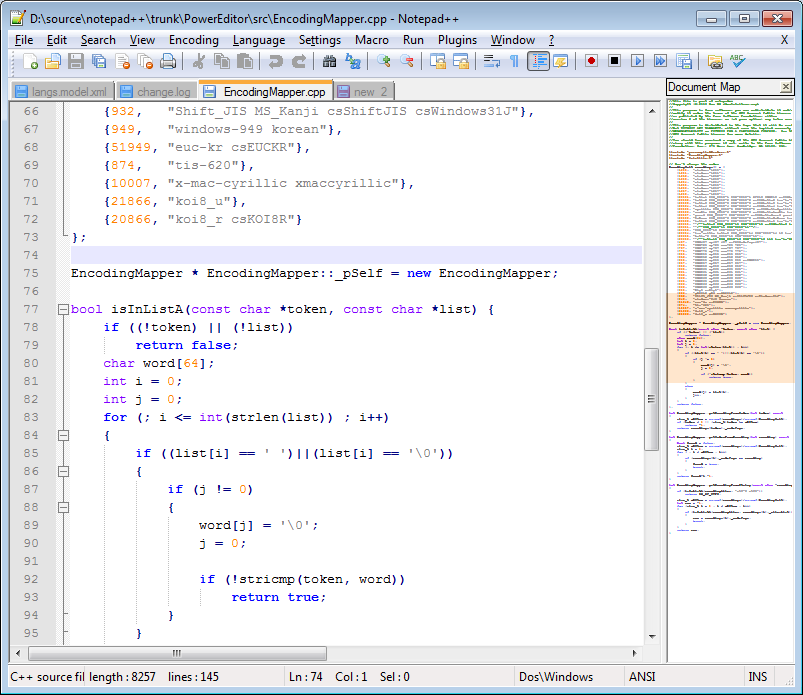
\includegraphics
   [width=\paperwidth]{images/notepad-plus-plus-screenshot.png}}
\begin{frame}[plain]%{RMS}
%  
\end{frame}
\setbeamertemplate{background canvas}{}

\setbeamertemplate{background canvas}{\centering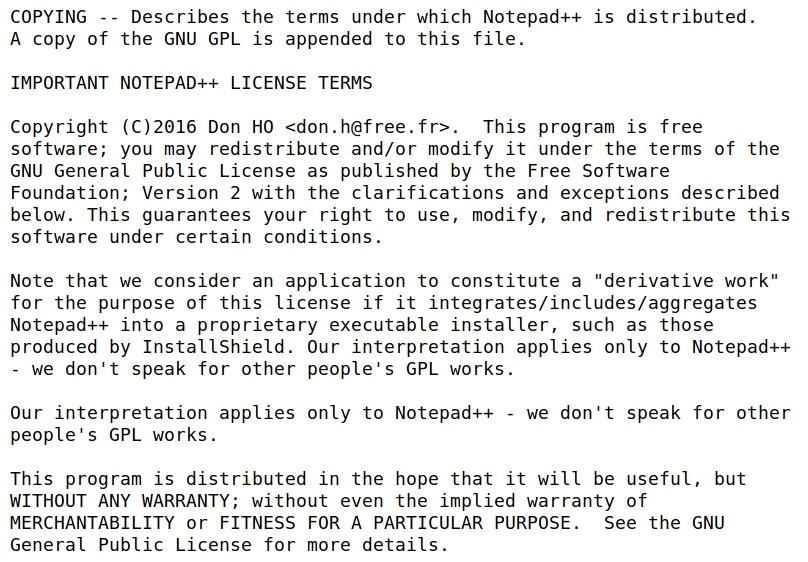
\includegraphics
   [width=\paperwidth]{images/notepad-plus-plus-LICENSE.jpg}}
\begin{frame}[plain]%{RMS}
%  
\end{frame}
\setbeamertemplate{background canvas}{}

\setbeamertemplate{background canvas}{\centering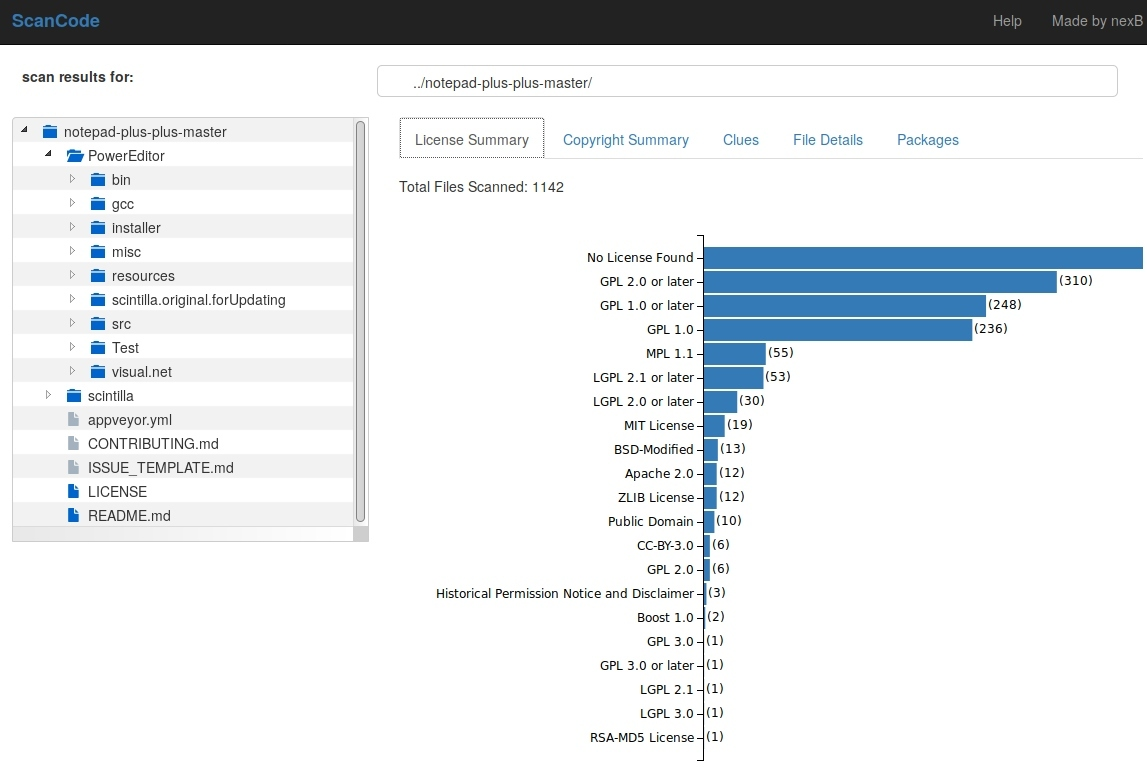
\includegraphics
   [width=\paperwidth]{images/notepad-plus-plus-scancode.jpg}}
\begin{frame}[plain]%{RMS}
%  
\end{frame}
\setbeamertemplate{background canvas}{}


\setbeamertemplate{background canvas}{\centering\includegraphics
   [width=\paperwidth]{images/scancode-ffmpeg.png}}
\begin{frame}[plain]%{RMS}
%  
\note{RMS}
\end{frame}
\setbeamertemplate{background canvas}{}

\setbeamertemplate{background canvas}{\centering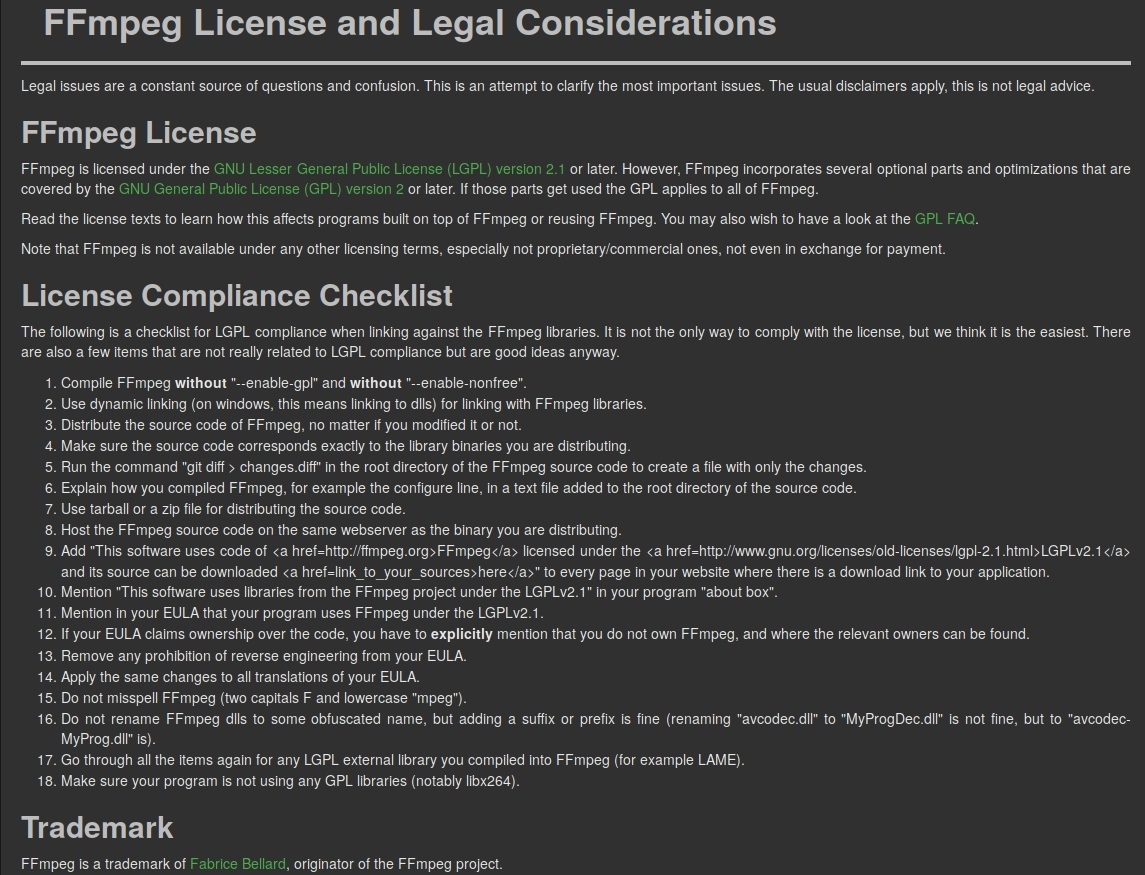
\includegraphics
   [width=\paperwidth]{images/FFmpeg-license-and-legal-consideration.jpg}}
\begin{frame}[plain]%{RMS}
%  
\note{RMS}
\end{frame}
\setbeamertemplate{background canvas}{}

\begin{frame}{Why do we have to care ?}
  \begin{alertblock}{Why do we have to care ?}
    \begin{itemize}
    \item Very rare to write a software \emph{from scratch...}
    \item A typical software project often reuses hundreds of
      third-party components...
    \item code quality if often much much better...
    \item you are a potential IT professional, so well, you MUST know a bit on that !
    \end{itemize}

\end{alertblock}
\end{frame}

%\section{Objectifs}

\begin{frame}
\frametitle{Your goal}
\begin{alertblock}{Main goal}
  Acquire and strengthen your expertise on free software licences
\end{alertblock}


  \begin{itemize}
  \item History and context
  \item Different families of licenses
  \item Diffusivity and compliance rules
  \item Auditing your project
  \item Free software economics
  \end{itemize}
\end{frame}

%%%%%%%%%%%%%%%%%%%%%%%%%%%%%%%%%%%%%%%%%%%%%%%%%%%%%%%%
% Context, vocabulary
%%%%%%%%%%%%%%%%%%%%%%%%%%%%%%%%%%%%%%%%%%%%%%%%%%%%%%%%

\section{Context}

\begin{frame}{Where does it come from ?}
  \begin{itemize}
  \item GNU project in 1984 by Richard Stallman (RMS)
  \item GPLv1 : 25th of february 1989
  %\item la technique est un moyen pour atteindre un but social
  \item 1991 : Linux based on Minix (\textit{just a hobby, won't be big and professional like gnu} by Linus Torvalds (LT)
  \item 1995 : Red Hat (NASDAQ in 1999), Apache license
  \item 1998 : release of Netscape source-code (fight back IE. Free the lizard, mozilla)
  \item 1998 : "Free software" versus "Open Source Software" (OSI). Rebranding the free software movement to emphasize the business potential ? 
  \end{itemize}
\end{frame}


\setbeamertemplate{background canvas}{\centering\includegraphics
   [width=\paperwidth]{images/rms.jpg}}
\begin{frame}[plain]%{RMS}
%  
\note{RMS}
\end{frame}
\setbeamertemplate{background canvas}{}


\setbeamertemplate{background canvas}{\centering\includegraphics
   [height=\paperheight]{images/LinusTorvalds.jpg}}
\begin{frame}[plain]%{LT}
%  
\note{Linus Torvalds}
\end{frame}
\setbeamertemplate{background canvas}{}

\setbeamertemplate{background canvas}{\centering\includegraphics
   [height=\paperheight]{images/gnu-linux_wallpaper_tb_david_revoy.png}}
\begin{frame}[plain]%{LT}
%  
\note{GNU/Linux}
\end{frame}
\setbeamertemplate{background canvas}{}

\begin{frame}{Communities and organizations}
  \begin{itemize}
  \item Free Software Fondation : \url{https://www.fsf.org/}
  \item Open Source Initiative : \url{https://opensource.org/}
  \item Linux Fondation : \url{https://www.linuxfoundation.org/}
  \item Debian, python, Ubuntu, KDE... communities
  \end{itemize}
\end{frame}


\begin{frame}{Why Free and/or Open Source Software ?}

  \begin{block}{Free Software}
    Social movement, user's essential freedom, free as in
    freedom. \textit{"political and ethical choice asserting the right
      to learn, and share what we learn with others"}
  \end{block}

  \textit{"All freedoms depend on freedom of information and are not
    more important than other fundamental freedoms, but as life's
    practices change over to the computer, it will be needed to
    maintain other freedoms". (RMS)}

  \pause

  \begin{block}{Open Source}
    Concerned solely with licensing of source code: \textit{"I think
      ideology sucks"} (Linus Torvalds), pragmatism.
  \end{block}

  We are always the ideologist of someone... Outdated debate ?
\end{frame}

\section{Vocabulary}


\begin{frame}{Vocabulary}
  \begin{itemize}
  \item \textbf{proprietary software} but all software have authors.
  \item \textbf{Copyright} : legal term describing rights given to
    creators for their works. Under the Berne Convention, everything
    written is automatically copyrighted from whenever it is put in
    \emph{fixed form}
  \item \textbf{Copyleft} :
    \begin{itemize}
    \item \textit{we give rights}, uses functional parts of copyright
      law to achieve a legal protection for free sharing (\emph{clever
        hack})
    \item all modified and extended versions of the program must be
      free as well, under the same terms.
    \item You cannot add restrictions to deny other people freedoms.
    \end{itemize}

  \end{itemize}
\end{frame}

\setbeamertemplate{background canvas}{\hspace{1.5cm}\centering\includegraphics%[scale=0.5]{images/Copyright.png}}
   [height=\paperheight]{images/Copyright.png}}
\begin{frame}[plain]%{LT}
%  
\end{frame}
\setbeamertemplate{background canvas}{}

\begin{frame}{Copyright}

With the creation authors obtain intellectual property rights.

  \begin{itemize}
  \item Economic rights :
    \begin{itemize}
    \item permit or prohibit the fixation and reproduction of their
      work
    \item translation, arrangement, adaptation and alteration of the
      work
    \item distribution of the original or copies
    \item Related rights
    \end{itemize}
  \item Moral right
    \begin{itemize}
    \item right to protect their personal connection with the work
    
    \end{itemize}
  \end{itemize}

 
  \begin{alertblock}{EU directive}
    \begin{itemize}
    \item the expression of a computer program is protected by
      copyright.
    \item ideas and principles which underlie any element of a
      program, including those which underlie its interfaces, are not
      protected by copyright.
    \end{itemize}

  \end{alertblock}

\end{frame}

\setbeamertemplate{background canvas}{\hspace{1.5cm}\centering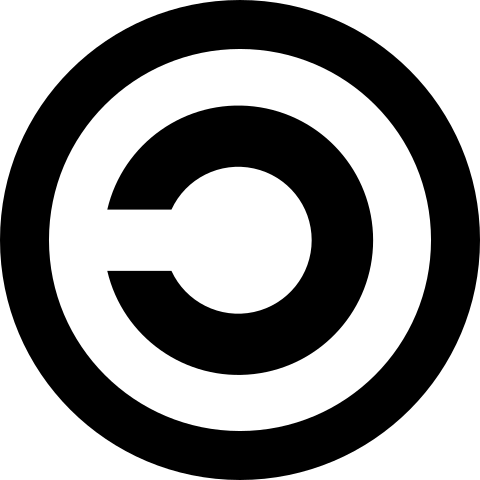
\includegraphics
   [height=\paperheight]{images/Copyleft.png}}
\begin{frame}[plain]%{LT}
%  
\end{frame}
\setbeamertemplate{background canvas}{}

\begin{frame}{Copyleft}

  \begin{block}{What is copyleft ?}
    Copyleft is a general method for making a program (or other work)
    free (in the sense of freedom, not “zero price”), and requiring
    all modified and extended versions of the program to be free as
    well.
  \end{block}

  \begin{block}{How to copyleft ?}
    we first state that it is copyrighted; then we add distribution
    terms, which are a legal instrument that gives everyone the rights
    to use, modify, and redistribute the program's code, or any
    program derived from it, but only if the distribution terms are
    unchanged.

    Thus, the code and the freedoms become legally inseparable.
  \end{block}

    
\end{frame}

%%%%%%%%%%%%%%%%%%%%%%%%%%%%%%%%%%%%%%%%%%%%%%%%%%%%%%%%
% Proprietary software
%%%%%%%%%%%%%%%%%%%%%%%%%%%%%%%%%%%%%%%%%%%%%%%%%%%%%%%%

\section{Proprietary}

\begin{frame}{Proprietary software}
  General principle : limitations against use, distribution and
  modification. Use by end-users only under predefined conditions.

  \begin{alertblock}{Definition : proprietary software}
    Software who limits at least one of the 4 freedoms of free
    software.
  \end{alertblock}

  \pause

  \begin{block}{Michel Rocard, 2002, patent battle : 648 no, 14 yes,
      18 abs}
    \textit{Creation, freedom, innovation were on the side of free
      software. The pursuit of profit, and above all the rent, the
      desire to restrict competition, and to restrain the external
      innovations, were on the side of big industry.}
  \end{block}
\end{frame}

%%%%%%%%%%%%%%%%%%%%%%%%%%%%%%%%%%%%%%%%%%%%%%%%%%%%%%%%
% Free software
%%%%%%%%%%%%%%%%%%%%%%%%%%%%%%%%%%%%%%%%%%%%%%%%%%%%%%%%

\section{Free Software}


\begin{frame}{Free Software}

  \begin{alertblock}{General principle}
    \textit{Free as in free speech, not as in free beer}. Source code
    is free.
  \end{alertblock}

  Their main difference is in the modalities of redistribution. In all
  cases source code must stay free. Two large families :

  \begin{enumerate}
  \item user's should receive a copy of the code under the same terms
    (GPL, LGPL, MPL...)
  \item user's are not guaranteed to receive a copy (BSDx, MIT...)
  \end{enumerate}

  \begin{alertblock}{Definition : free software}
    A program is free software if the \textbf{program's users} have
    the four essential freedoms.
  \end{alertblock}
  
\end{frame}

% Not the canonical order :
% see https://www.softwarefreedom.org/resources/2014/SFLC-Guide_to_GPL_Compliance_2d_ed.html#copyright-and-copyleft

\subsection{4 freedoms}


\begin{frame}{freedom 0 : freedom to run the program}
  \begin{itemize}
  \item Absolute freedom to run by anyone without \textbf{any} restriction
  \item A work produced with a free software doesn't have to be free
  \item Some production made by a free software could been seen as a derivative work (compiler mostly).
  \item What about SaaS ?
  \end{itemize}

  \begin{alertblock}{Principle}
     it is the user's purpose that matters (all users not only developer's one).
  \end{alertblock}
  
  Quick question : Is JSON license free ? \url{http://www.json.org/license.html}

\end{frame}


\begin{frame}{freedom 1 : freedom to study}
  \begin{itemize}
  \item study without any obstacles (technicals, rights...)
  \item includes the freedom to use your modified version in place of the original one
  \item Source code should be made available for free or at a low cost
  \item Source code available for at least 3 years (GPLv3)
  \end{itemize}
  \begin{alertblock}{Principe}
    Again, it is the user's purpose that matters, not the developer's one
  \end{alertblock}
\end{frame}


\begin{frame}{freedom 2 : freedom to modify}
  \begin{itemize}
  \item absolute freedom. Only restrictions when distribution.
  \item Preserve copyritht ownership (Berne convention)
  \item Identify  contributions
  \end{itemize}
\begin{alertblock}{Principe}
    Always, it is the user's purpose that matters
  \end{alertblock}
\end{frame}

\begin{frame}{freedom 3 : freedom to redistribute}

Anyone, anywhere (export control, trade sanctions...)

  \begin{itemize}
  \item Conditions of redistribution : main difference between all free software licenses :
    \begin{itemize}
    \item \textbf{Copyleft (strong or weak)}
    \item \textbf{Copyfree}
    \end{itemize}
  \item Always identify contributors (Berne convention)
  \item Preserve original authors' reputation
  \end{itemize}
\begin{alertblock}{Principle}
    User's purpose again and mostly necessary condition for the three others freedoms.
  \end{alertblock}

\begin{alertblock}{When does license apply ?}
\textbf{Redistribution triggers !}
 \end{alertblock}
 
 Exception : APGL 
\end{frame}

\begin{frame}
  Questions ?
\end{frame}

\section{Bibliography and credits}

\begin{frame}{References}

Bibliography (in french) :

  \begin{itemize}
  \item "Droit des logiciels, logiciels proprietaires, logiciels libres", F.Pellegrini et S.Canevet, PUF 2013.
  \item "Option libre. Du bon usage des licenses libres", B.Jean, Framabook 2012.
  \item "Histoire et cultures du Libre. Des logiciels partagés aux licenses partagés", Collectif, Framabook 2013.
  \end{itemize}

Websites :

\begin{itemize}
\item \url{http://gplv3.fsf.org/}
\item \url{https://copyleft.org/guide/}
\item \url{http://april.org/en}
\end{itemize}
  
\end{frame}

\begin{frame}{Credits 1/2}
  \begin{itemize}
  \item Photo of Richard Stallman by Lionel Allorge, license GFDL1.3+, CC-BY-SA+, LAL+,  \url{http://photos.april.org/picture.php?/4413/category/159}
  \item Photo of Linus Torvalds from Wikimedia Commons, license CC-BY-SA 3.0 capture d'une vidéo de Linux Foundation Kernel Summit 2008 \url{https://upload.wikimedia.org/wikipedia/commons/3/31/Linus_Torvalds_lks08.jpg}
  \item GNU/Linux, David Revoy, CC-BY \url{http://deevad.deviantart.com/art/GNU-Linux-Portrait-645635708}
  
  \end{itemize}
\end{frame}

\begin{frame}{license}
  Document under GFDL1.3+, CC-BY-SA+, LAL+.
\end{frame}

\end{document}

%%% Local Variables:
%%% mode: latex
%%% TeX-master: t
%%% End:
